% Research report, max 3 pages. Build: pdflatex report.tex (twice, for hyperref).
% Figures: put frames from the three rollout videos in docs/figures/ (names below).
% Missing figures are replaced by a grey placeholder box, so the file always compiles.
\documentclass[10pt,a4paper]{article}
\usepackage[margin=1.6cm,top=1.4cm,bottom=1.4cm]{geometry}
\usepackage[T1]{fontenc}
\usepackage{lmodern,microtype}
\usepackage{graphicx,booktabs,tabularx,enumitem,xcolor}
\usepackage{tikz}
\usetikzlibrary{positioning,arrows.meta,fit,backgrounds}
\usepackage[colorlinks=true,urlcolor=blue!60!black,linkcolor=blue!60!black,citecolor=blue!60!black]{hyperref}
\usepackage[font=footnotesize,labelfont=bf,skip=2pt]{caption}

\setlist{nosep,leftmargin=1.2em}
\setlength{\parindent}{0pt}
\setlength{\parskip}{2pt}
\usepackage{titlesec}
\newcommand{\key}[1]{#1}% marks key phrases; set to \textbf{#1} or \uline{#1} (with ulem) to highlight
\titleformat{\section}{\large\bfseries}{\thesection}{0.5em}{}
\titleformat{\subsection}{\normalsize\bfseries}{\thesubsection}{0.5em}{}
\titlespacing*{\section}{0pt}{6pt}{2pt}
\titlespacing*{\subsection}{0pt}{4pt}{1pt}

% Branch that holds docs/videos. Change to master after merging.
\newcommand{\repo}{https://github.com/tkpf/dual-system-architecture-vla/blob/finetune}
\newcommand{\vid}[2]{\href{\repo/docs/videos/#1}{#2}}

% figure helper: shows the image if present, else a placeholder
\newcommand{\fig}[3]{% file, width, (unused)
  \IfFileExists{figures/#1}{\includegraphics[width=#2]{figures/#1}}%
  {\fbox{\parbox[c][2.6cm][c]{#2}{\centering\footnotesize\color{gray}missing: figures/\detokenize{#1}}}}}

\newcolumntype{Y}{>{\centering\arraybackslash}X}
\renewcommand{\arraystretch}{1.1}

\begin{document}

\begin{center}
{\LARGE\bfseries Dual-System VLA on LIBERO}\\[3pt]
\small Code, videos and experiment log: \href{https://github.com/tkpf/dual-system-architecture-vla}{github.com/tkpf/dual-system-architecture-vla}
\end{center}

\section*{Task}
A Dual-System policy for the LIBERO benchmark is to be built. System~2 (slow, semantic) conditions System~1 (fast, reactive). An ablation must show whether System~2 really improves System~1. Hi~Robot \cite{hirobot} served as role model: a high level writes text commands, a low-level VLA executes them.

\begin{table}[h]
\centering\footnotesize
\begin{tabularx}{\linewidth}{@{}lX@{}}
\toprule
\multicolumn{2}{@{}l}{\textbf{Key results at a glance}}\\
\midrule
Counterfactual & Removing System~2 does \key{not} hurt: 9/20 without it, 4/20 with it (\texttt{libero\_10}). Freezing it hurts (1/4).\\
Error recovery & Drops are detected in 8/8 cases. Success is \key{unchanged} with and without recovery (6/8 each).\\
Bottleneck & \key{Execution}, not reasoning: 13 of 16 failures also fail under oracle switching.\\
\bottomrule
\end{tabularx}
\end{table}

\section{Prerequisites}
\begin{itemize}
\item \emph{No private GPU.} Surface Laptop Studio, Intel Iris Xe, 16~GB RAM, no CUDA.
\item \emph{One week} for design, experiments and report.
\item \emph{Little experience} with VLMs and VLAs.
\end{itemize}

\section{Tools}
\begin{itemize}
\item \emph{Google Colab:} T4 and L4 GPUs for all evaluation.
\item \emph{Colab MCP server:} lets the coding agent drive a Colab notebook.
\item \emph{Coding LLMs:} Claude Sonnet 5.5 and Opus 5.5.
\end{itemize}

\subsection*{Models used and investigated}
\begin{table}[h]
\centering\scriptsize
\begin{tabularx}{\linewidth}{@{}p{2.1cm}p{2.6cm}p{5.6cm}X@{}}
\toprule
Model & Role & Checkpoint & Status\\
\midrule
pi0.5 & System 1, final & \path{lerobot/pi05_libero_finetuned_v044} & Used frozen. Finetuned for 400 steps: no gain\\
\midrule
SmolVLA & System 1, v1 & \path{lerobot/smolvla_libero_plus} (finetuning started from \path{lerobot/smolvla_libero}) & Replaced by pi0.5. Finetuned for 600 steps: no gain\\
\midrule
Qwen3-VL 2B & System 2 VLM, final & \path{Qwen/Qwen3-VL-2B-Instruct} & Used frozen, for act phases only\\
\midrule
Qwen3-VL 4B, 8B & Offline judge tests & \path{Qwen/Qwen3-VL-4B-Instruct}, \path{Qwen/Qwen3-VL-8B-Instruct} & Investigated: not reliable enough\\
\midrule
SmolVLM2 2.2B & Offline judge tests & \path{HuggingFaceTB/SmolVLM2-2.2B-Instruct} & Investigated: not better\\
\bottomrule
\end{tabularx}
\caption{Models. Software: LeRobot 0.6.1 with the official LIBERO pipeline.}
\label{tab:models}
\end{table}

\section{Architecture}\label{sec:design}
\subsection{Generic design: frozen VLM and VLA, joined by text}
\begin{itemize}
\item \emph{Both models are frozen.} System~2 writes \emph{one English sentence} into System~1's prompt.
\item \key{Interpretable.} The interface is readable text. No latent embedding sits in between.
\item \emph{Easy to ablate.} System~2 can be removed, frozen, replaced by an oracle or corrupted. Nothing is retrained.
\item \emph{No training needed.} This fits the compute and time budget.
\item \emph{Price:} neither side can adapt to the other. Section~\ref{sec:evolution} shows where this limit bit.
\end{itemize}

\subsection{How the implementation evolved}\label{sec:evolution}
The generic design never changed. Two things changed: \emph{when} System~2 runs and \emph{who judges progress}.

\begin{table}[h]
\centering\scriptsize
\begin{tabularx}{\linewidth}{@{}p{1.7cm}p{3.6cm}p{3.5cm}X@{}}
\toprule
Version & System 2 runs & Progress judged by & Outcome\\
\midrule
v1: SmolVLA, VLM judge & Every 20 steps, plus environment triggers (gripper toggle, robot stops, empty grasp, 300-step timeout) & Qwen3-VL 2B: running, done or failed. ``Success'' ends the episode & Success 19/36 $\to$ 4/36. 7 of 11 success verdicts were wrong\\
\midrule
v2: pi0.5 as System 1 & Same triggers & Same VLM judge & pi0.5 follows commands (16/17 against 3/17 for gibberish). Dual still worse: 8/12 $\to$ 3/12\\
\midrule
v3: phase-aware prompt & Triggers, 150-step timeout & VLM told phase and ``done'' criteria, short reasoning & No false successes, but 0 ``done'' in 76 checks\\
\midrule
\key{v4: final} & \emph{Every step} on robot signals. VLM every 10 steps, act phases only & \emph{Gripper width and hand height}; VLM only for ``turn on'', ``open'', ``close'' & Matches oracle switching. Never ends an episode\\
\bottomrule
\end{tabularx}
\caption{Evolution of System~2. The generic design is identical in all rows.}
\label{tab:evolution}
\end{table}

\emph{What the failures showed:}
\begin{enumerate}
\item \emph{SmolVLA ignores language.} Gibberish gave the same behaviour as real commands. pi0.5 replaced it.
\item \emph{Finetuning System~1 on subtasks did not help.} pi0.5 reached 17/28 goals against 21/28 stock. Both policies stay frozen.
\item \key{The VLM judge is the weak part.} No untrained VLM up to Qwen3-VL~8B judged ``finished'' reliably (best AUROC 0.71, about 1/3 false ``done''). Qwen~2B calls a glowing burner dark.
\item \emph{Hence v4:} the progress check moved to robot signals. The VLM is kept only where no signal exists.
\end{enumerate}

\subsection{Final architecture}
\begin{figure}[h]
\centering
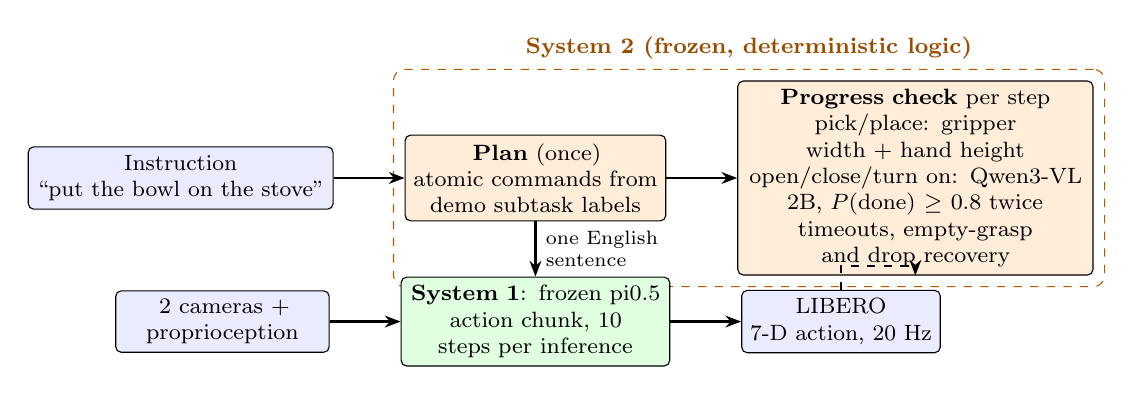
\begin{tikzpicture}[
  node distance=5mm and 9mm,
  box/.style={draw,rounded corners=2pt,fill=#1,align=center,font=\footnotesize,inner sep=3pt,minimum height=7mm},
  box/.default=white,
  arr/.style={-{Stealth[length=2mm]},thick}]
\node[box=blue!8] (instr) {Instruction\\``put the bowl on the stove''};
\node[box=orange!15,right=of instr,text width=3.1cm] (plan) {\textbf{Plan} (once)\\atomic commands from demo subtask labels};
\node[box=orange!15,right=of plan,text width=4.3cm] (sw) {\textbf{Progress check} per step\\pick/place: gripper width + hand height\\open/close/turn on: Qwen3-VL 2B, $P(\mathrm{done})\!\ge\!0.8$ twice\\timeouts, empty-grasp and drop recovery};
\node[box=green!12,below=7mm of plan,text width=3.2cm] (s1) {\textbf{System 1}: frozen pi0.5\\action chunk, 10 steps per inference};
\node[box=blue!8,left=of s1,text width=2.5cm] (obs) {2 cameras +\\proprioception};
\node[box=blue!8,right=of s1] (env) {LIBERO\\7-D action, 20~Hz};
\begin{scope}[on background layer]
\node[draw=orange!70!black,dashed,rounded corners,fit=(plan)(sw),inner sep=4pt,label={[font=\footnotesize\bfseries,orange!60!black]above:System 2 (frozen, deterministic logic)}] {};
\end{scope}
\draw[arr] (instr) -- (plan);
\draw[arr] (plan) -- (sw);
\draw[arr] (obs) -- (s1);
\draw[arr] (s1) -- (env);
\draw[arr] (plan) -- node[right,font=\scriptsize,align=left]{one English\\sentence} (s1);
\draw[arr,dashed] (env.north) |- ++(0,3mm) -| (sw.south);
\end{tikzpicture}
\caption{Final system. A changed command clears System~1's queued actions. Dashed: gripper and camera signals feed the progress check.}
\label{fig:arch}
\end{figure}

\begin{itemize}
\item \emph{Pick done:} gripper holds something for 8 steps and the hand rose 3~cm.
\item \emph{Place done:} gripper reopens after a hold.
\item \emph{Timeout:} 150 steps per phase.
\item \emph{Empty grasp:} ``open the gripper'', then retry.
\end{itemize}

\section{Ablation}
\emph{Protocol:} same scene, robot start and seed for every condition. Shifted starts move the gripper by about 10~cm (C) or 19~cm (B).
\begin{table}[h]
\centering\footnotesize
\begin{tabularx}{\linewidth}{@{}lX@{}}
\toprule
Condition & Meaning\\
\midrule
passthrough & System~2 removed. The whole instruction is the prompt.\\
frozen & System~2 frozen. First atomic command for the whole episode.\\
fused & Final System~2.\\
oracle & Simulator decides when a phase is done. Upper bound for any progress check.\\
\bottomrule
\end{tabularx}
\end{table}

\subsection{Counterfactual: is System 2 needed?}
\begin{table}[h]
\centering\footnotesize
\begin{tabularx}{\linewidth}{lYYY}
\toprule
Condition & \texttt{libero\_goal}, 4 runs (median steps) & \texttt{libero\_10}, 10 scenes $\times$ 2 seeds, start B & Drop test, 8 episodes\\
\midrule
passthrough & 4/4 (99) & \key{9/20} & 5/8\\
frozen & 1/4 (218) & 7/20 & ---\\
fused & 4/4 (101) & 4/20 & 6/8\\
oracle & 4/4 (102) & 5/20 & 5/8\\
\bottomrule
\end{tabularx}
\caption{Success counts. Drop test: section~\ref{sec:recovery}.}
\label{tab:main}
\end{table}
\begin{itemize}
\item \key{Frozen System~2 fails:} the bowl is held, never placed (1/4).
\item \key{Fused $\approx$ oracle:} switches 0--2 steps from simulator truth. Same outcome in 15 of 20 pairs.
\item \key{System~2 does not beat passthrough.} Oracle also drops to 5/20.
\item \emph{Likely cause:} bare atomic commands are out of distribution for pi0.5. It was trained on whole instructions.
\item \emph{Significance:} none. Passthrough against fused: 7 against 2 pairs, $p{=}0.18$.
\item \emph{Consistency:} both seeds agree in 9/10 scenes with the whole instruction, in 5--6/10 with atomic commands.
\end{itemize}

\subsection{Error recovery}\label{sec:recovery}
\emph{Perturbation:} after 20 steps of holding, the gripper is forced open for 10 steps. The bowl falls. Two bowl scenes, start C, 4 seeds.
\begin{itemize}
\item \key{Detection works:} 8 of 8 drops found within 1--3 steps of the simulator.
\item \key{Recovery changes nothing:} fused with and without recovery fail on the same episodes (6/8 each).
\item \emph{Oracle recovery is no better:} 5/8.
\item \emph{Reason:} pi0.5 picks a dropped bowl up again by itself, even under ``place''.
\end{itemize}

\subsection{Bottleneck: reasoning or execution?}
\emph{Method:} each failed fused episode is checked against oracle switching on the same scene, start and seed.
\begin{table}[h]
\centering\footnotesize
\begin{tabularx}{\linewidth}{@{}lYX@{}}
\toprule
Failure source & Count & Evidence\\
\midrule
\key{Execution (System~1)} & 13 of 16 & Oracle fails too. No better progress check helps.\\
System~2 or rollout noise & 3 of 16 & Oracle succeeds. One case inspected (book scene): switches 1 step apart, outcome flipped in the other seed.\\
\bottomrule
\end{tabularx}
\end{table}


\begin{figure}[t]
\centering
\begin{tabular}{@{}ccc@{}}
\fig{goal_bowl_C.png}{0.30\linewidth}{} &
\fig{stove_moka_B.png}{0.30\linewidth}{} &
\fig{drop_bowl_C.png}{0.30\linewidth}{}\\[-1pt]
\vid{libero_goal_bowl_on_stove_C.mp4}{\footnotesize Video 1: easy scene} &
\vid{libero_10_stove_moka_B.mp4}{\footnotesize Video 2: stove, then moka pot} &
\vid{drop_bowl_on_stove_C.mp4}{\footnotesize Video 3: forced drop}
\end{tabular}
\caption{Frames from the 2$\times$2 rollout videos (top: passthrough, frozen; bottom: fused, oracle; each panel shows the command System~2 sends). (1) Frozen holds the bowl and never places it. (2) Atomic commands succeed where the whole instruction fails. (3) Fused notices the drop and re-commands the pick (frozen panel empty, not run). Captions link to the videos.}
\label{fig:videos}
\end{figure}

\section{Limitations and conclusion}
\subsection{Limitations}
\begin{itemize}
\item \emph{Small samples:} 20 scene-seed pairs, 8 drop episodes, one init state.
\item \emph{Out-of-distribution sensitivity:} results depend on the robot start and the seed. Another robot or scene would likely behave differently.
\item \emph{System~1 follows language only weakly.} The open-source VLAs probably overfit LIBERO and generalize poorly. This is a likely cause, not a tested one.
\item \emph{System~2 was not fully exercised:} the plan came from demo subtask labels. Qwen's own decomposition matched the reference in only 3 of 4 \texttt{libero\_goal} and 4 of 10 \texttt{libero\_10} episodes. Reliable verbal task splitting by a VLM is therefore not shown.
\end{itemize}

\subsection{Conclusion}
\begin{itemize}
\item The frozen, text-interfaced Dual System is fully interpretable.
\item System~2 matches an oracle at command switching and at drop detection.
\item An improvement over System~1 alone could not be shown.
\item With pi0.5, execution under atomic commands is the bottleneck, not reasoning.
\item System~2 could not be used as intended. It was engineered for switching accuracy, and the true subtasks were injected in the final run.
\end{itemize}

\subsection{What I would do next}
\begin{itemize}
\item \emph{Without training budget:} the choice was frozen models, because training outcomes are risky.
\item \emph{With more time and compute:} a diffusion policy that draws (dashed) bounding boxes around objects and place locations. These would be fed into a finetuned VLA.
\item \emph{Expected gain:} a more precise System~1 response.
\item \emph{Risk:} the VLA may rely on the boxes and obey language even less. The boxes can also be seen as a redundant second channel.
\end{itemize}


\begin{thebibliography}{9}\footnotesize
\bibitem{hirobot} L.~X. Shi et al. \emph{Hi Robot: Open-Ended Instruction Following with Hierarchical Vision-Language-Action Models}, arXiv:2502.19417, 2025.
\end{thebibliography}

\end{document}
